\chapter*{Appendices}
\addcontentsline{toc}{chapter}{Appendices}

\section*{User Interface Screenshots}

\subsection*{Landing Page}

\begin{figure}[H]
  \centering
  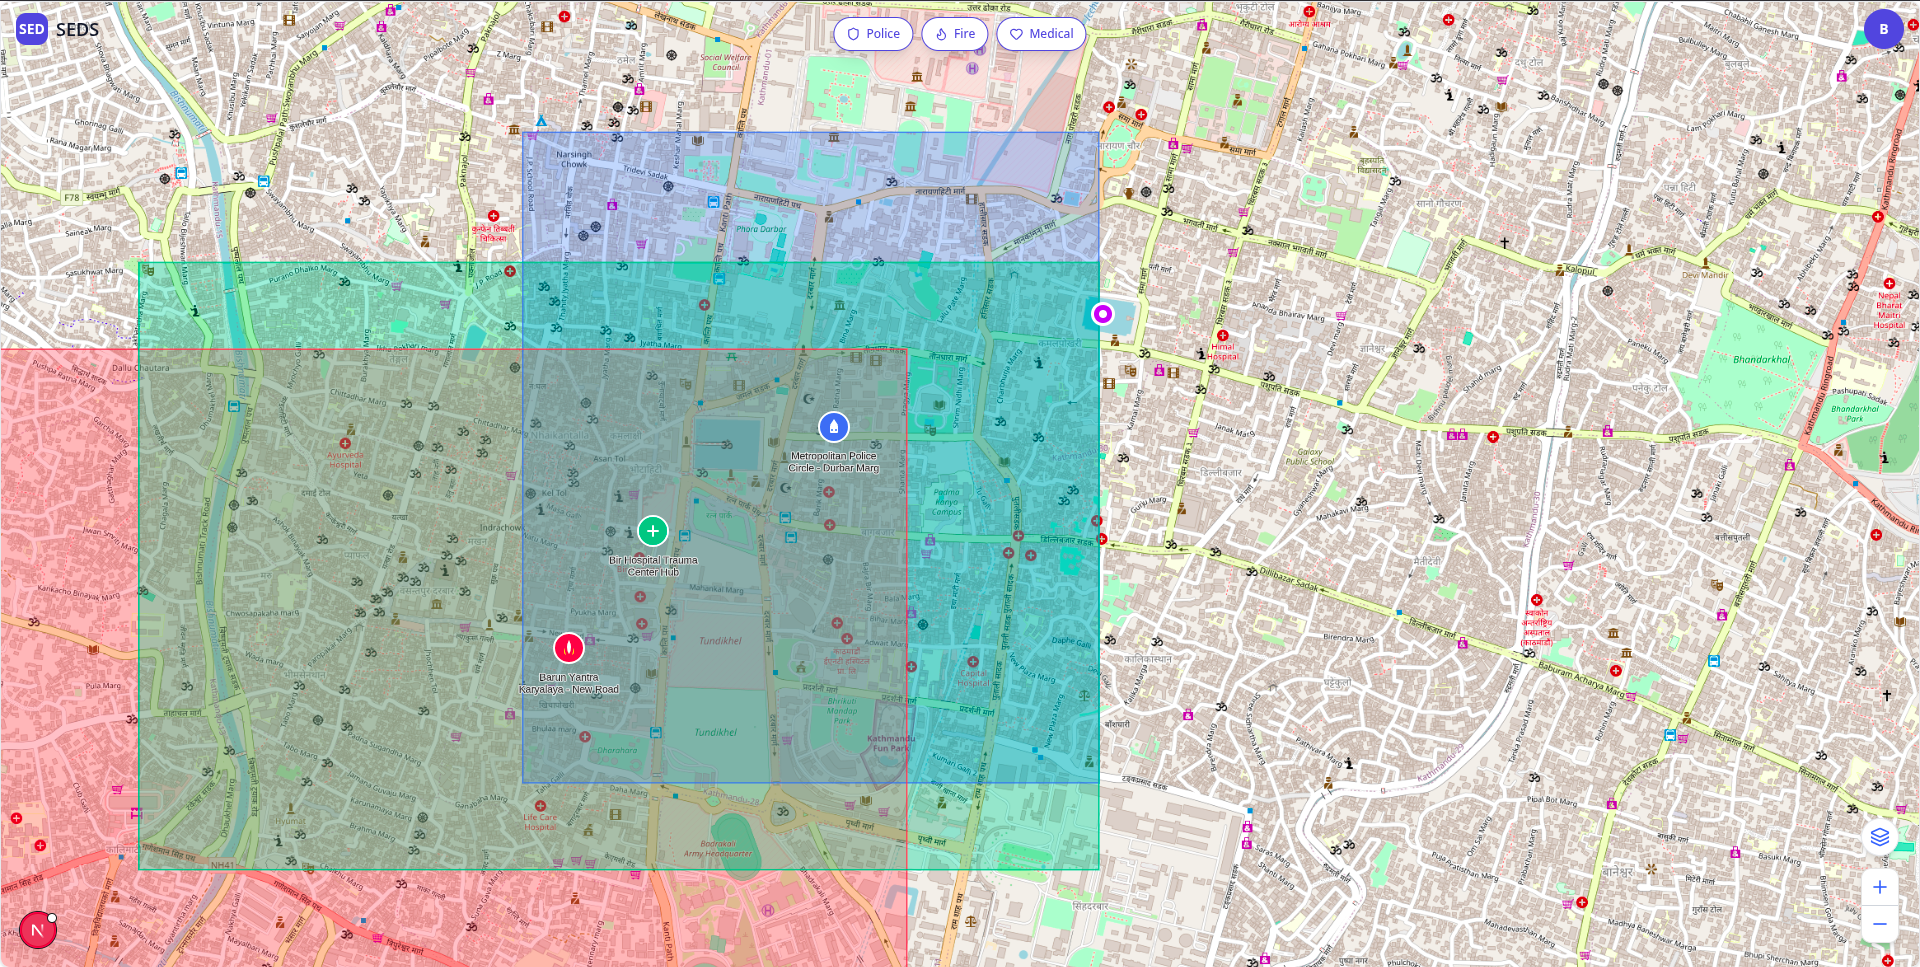
\includegraphics[width=0.95\textwidth]{Graphics/landing-page.png}
  \caption{Landing Page - Interactive map with stations and service zones}
  \label{fig:landing-page}
\end{figure}

The landing page provides an interactive map view of the emergency dispatch system. It displays all registered stations with their service zones represented as colored polygons on the map. Users can navigate the map, zoom in/out, and view detailed information about each station by clicking on them.

\FloatBarrier

\subsection*{Login Page}

\begin{figure}[H]
  \centering
  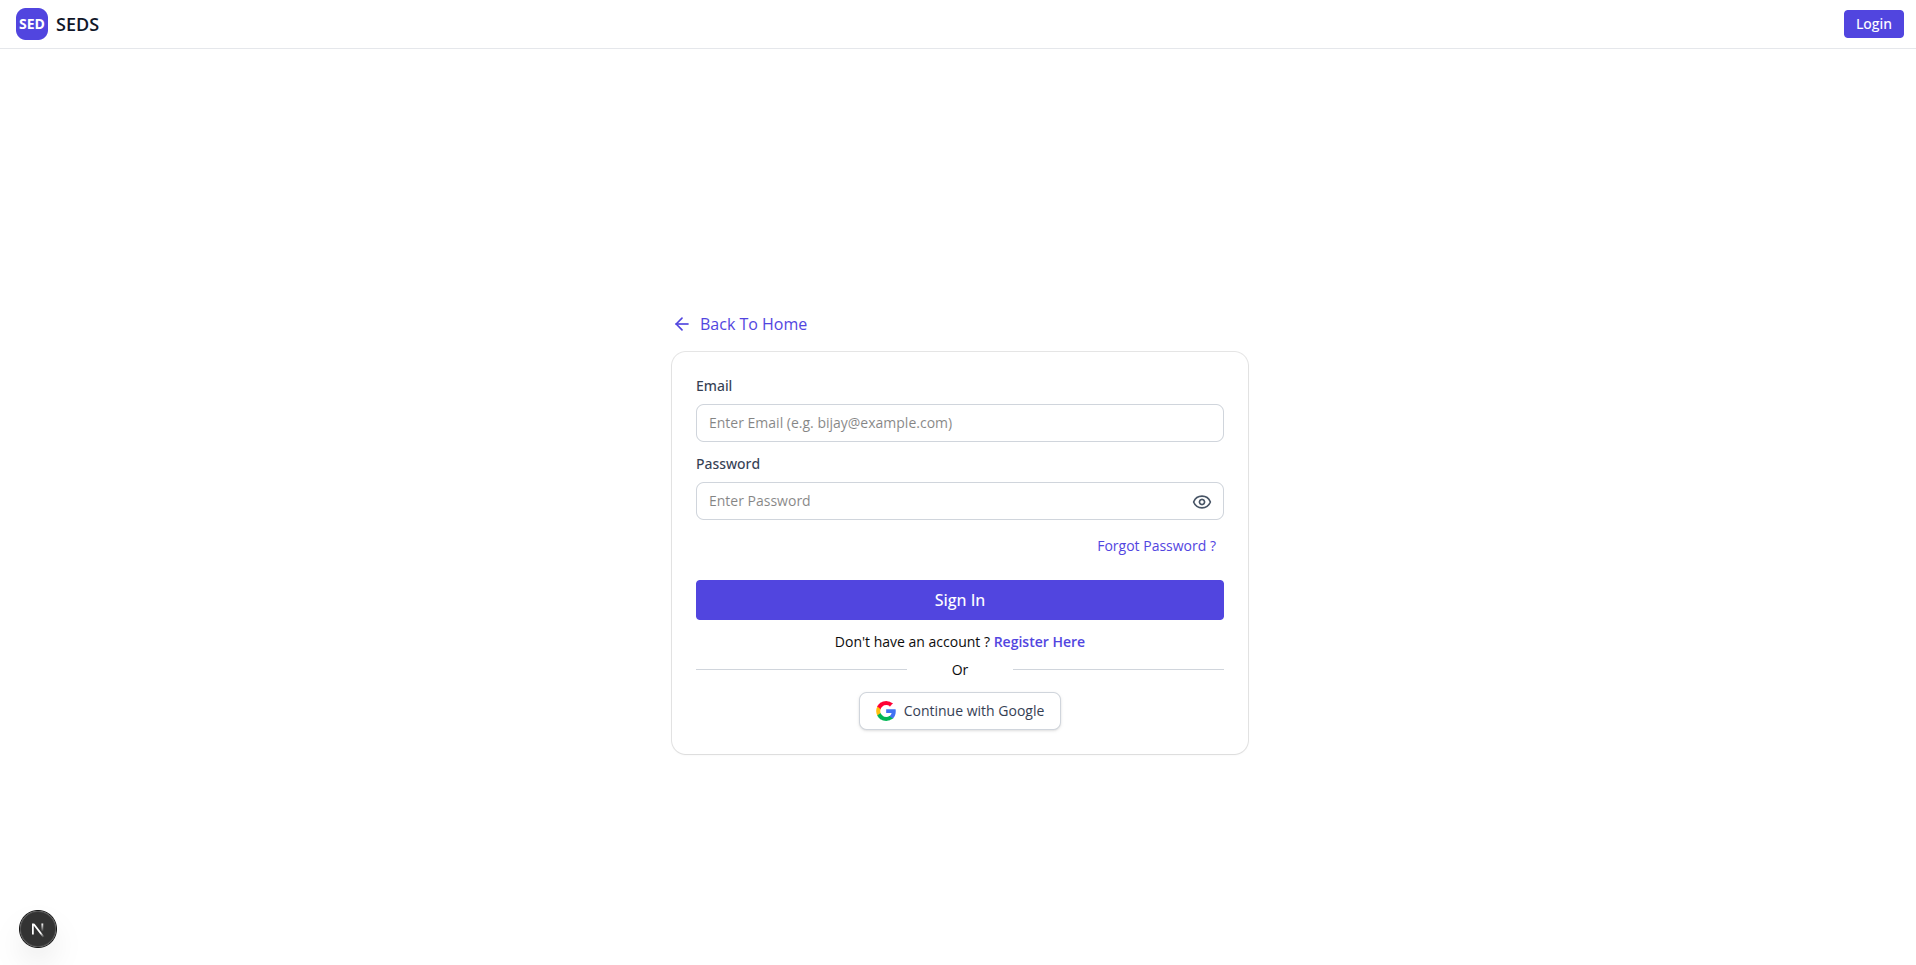
\includegraphics[width=0.6\textwidth]{Graphics/login-page.png}
  \caption{Login Page - Role-based authentication (Admin/Responder)}
  \label{fig:login-page}
\end{figure}

The login page provides a secure authentication interface for both administrators and emergency responders. Users can select their role from a dropdown menu and enter their credentials to access the system. Role-based access control ensures that each user sees only the relevant features and data for their role.

\FloatBarrier

\subsection*{Admin Dashboard}

\begin{figure}[H]
  \centering
  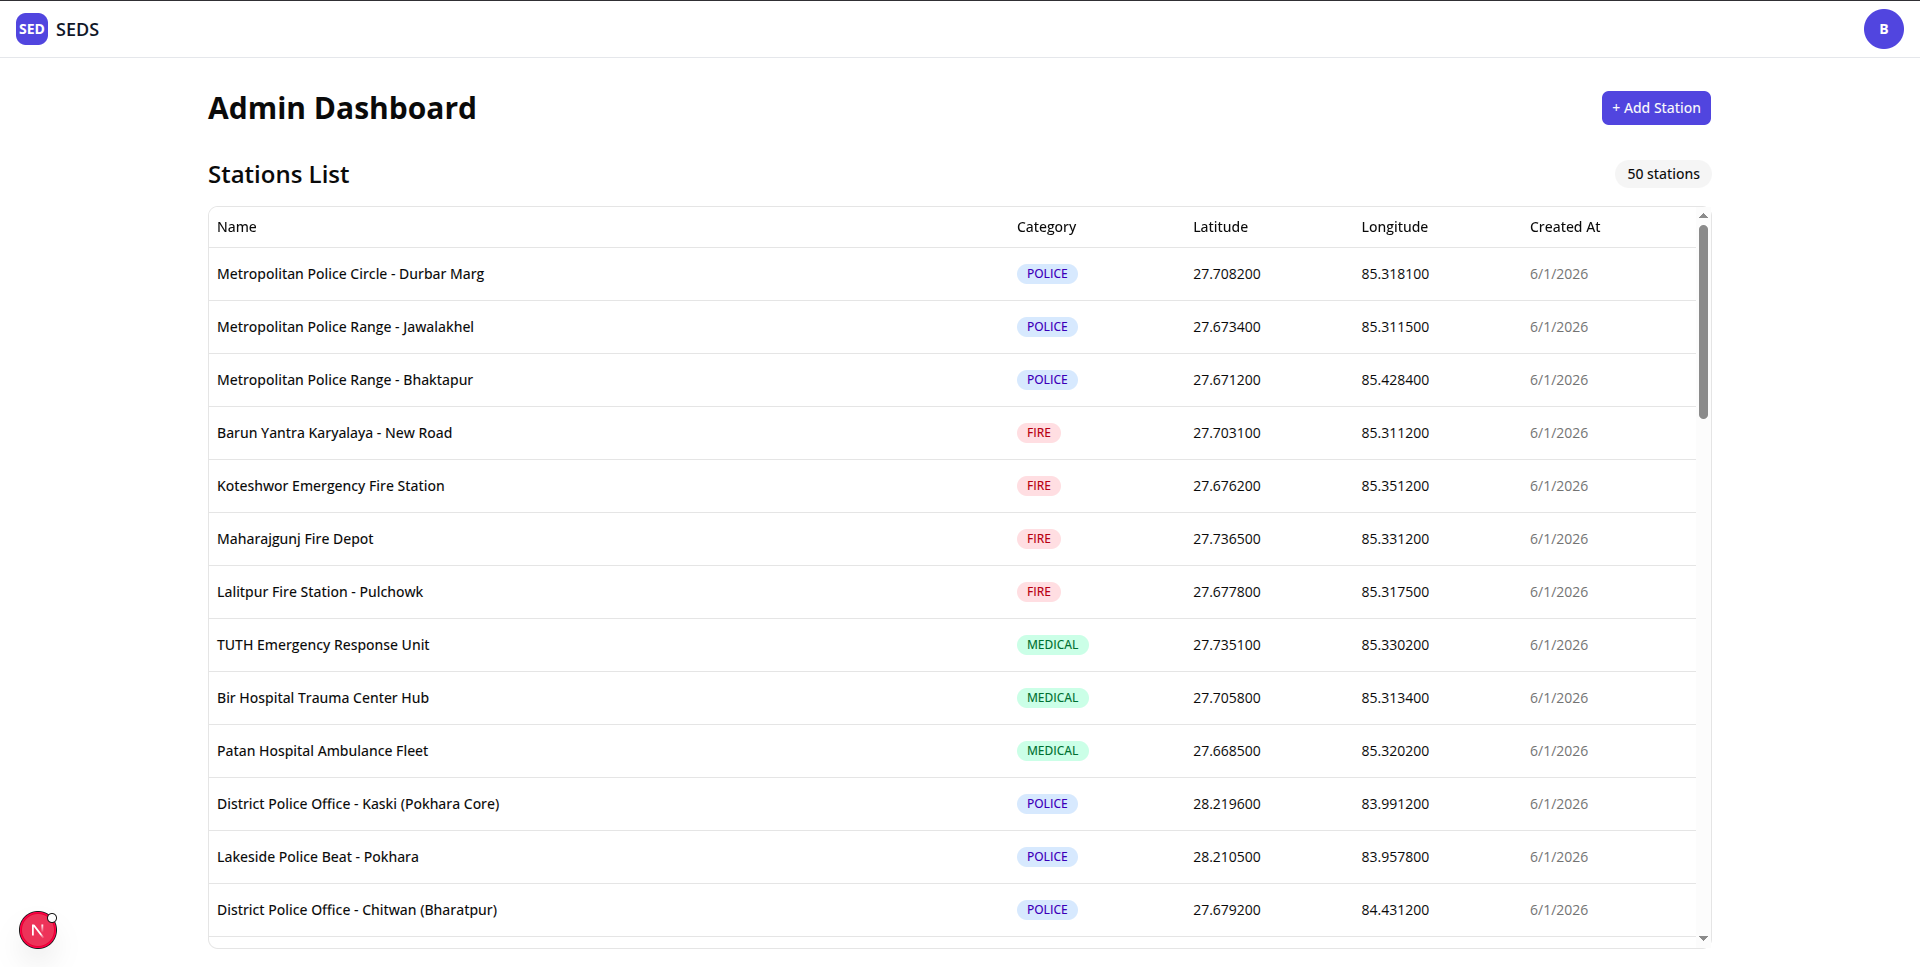
\includegraphics[width=0.95\textwidth]{Graphics/admin-dashboard.png}
  \caption{Admin Dashboard - Station management with CRUD operations}
  \label{fig:admin-dashboard}
\end{figure}

The admin dashboard provides comprehensive station management capabilities. Administrators can create new stations, update existing station information, delete stations, and manage responders assigned to each station. The dashboard displays a list of all stations with their current status and available responders.

\FloatBarrier

\subsection*{Add Station Form}

\begin{figure}[H]
  \centering
  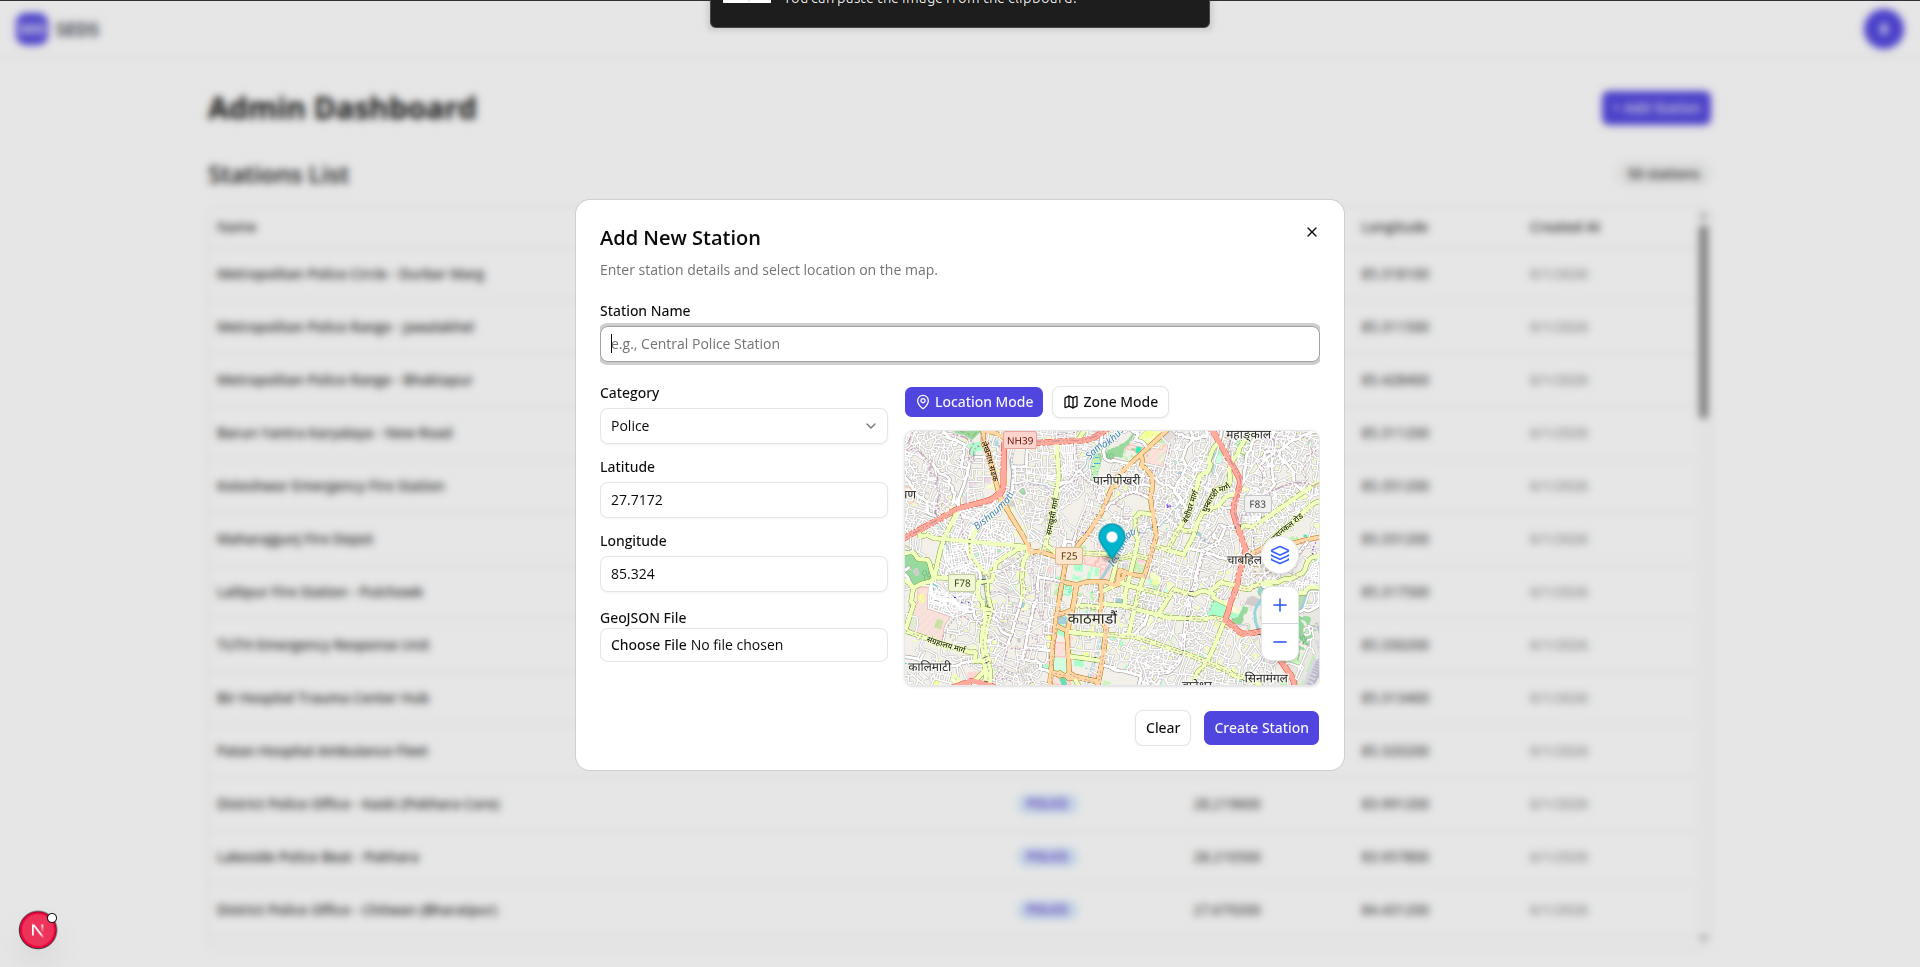
\includegraphics[width=0.75\textwidth]{Graphics/add-station-form.png}
  \caption{Add Station Form - Location picker and zone polygon drawing}
  \label{fig:add-station-form}
\end{figure}

The Add Station Form allows administrators to register new emergency response stations. It features an interactive map for selecting station location and a polygon drawing tool for defining the service zone boundary. The form validates all required fields including station name, category, and location coordinates before submission.

\FloatBarrier
